\def\QRCODE{MASTER_mispa_TUT.IMG.gaussian_random_fields_pythonqrcode.png}
\def\QRPAGE{http://www.iptutorials.science/tree/master/MASTER_mispa/TUT.IMG.gaussian_random_fields/python}
\def\difficulty{3}
\mcorrectionsection{Python correction}

\subsection{White noise}
The white noise is generated with the following code.
\begin{python}
%% white noise simulation
W = np.random.randn (N, N) ;
\end{python}

\subsection{Gaussian Random Field}
The Gaussian function that will serve as a covariance function is generated via the given code. Pay attention to the discretization grid: 
the FFT implies that functions are periodic, and in order to do that, the discretization must be set between $[-N/2:N/2[$.


The Gaussian Random Field can be generated via the formula already presented (see Fig.\ref{fig:grf:python:grf}).
\begin{python}
def grf2D(N, sigma):
    # Discrete space
    x = np.arange(-N/2 , N/2) ;
    [ X , Y ] = np.meshgrid( x , x ) ;
    # Covariance function
    C = np.exp(-1/2 * ( (X/ sigma /np.sqrt(2))**2+(Y/sigma/np.sqrt(2) )** 2 ) ) ;
    Cmat = np.fft.fftshift (C) ;
    # real positive part, then square root
    Cf = np.real(np.fft.fft2( Cmat ) ) ;
    Cf = np.sqrt ( np.maximum ( np.zeros ( Cf.shape ) , Cf ) ) ;
    # Complex white noise
    W = np.random.randn (N, N) ;
    
    A = Cf * np.fft.fft2(W);
    G = np.real ( np.fft.ifft2 (A) ) ;
    return G;
\end{python}

\begin{figure}[htbp]
 \centering\caption{Gaussian Random Field, with $\sigma=10$ (pixels) and $N=2^{10}=1024$ pixels.}%
 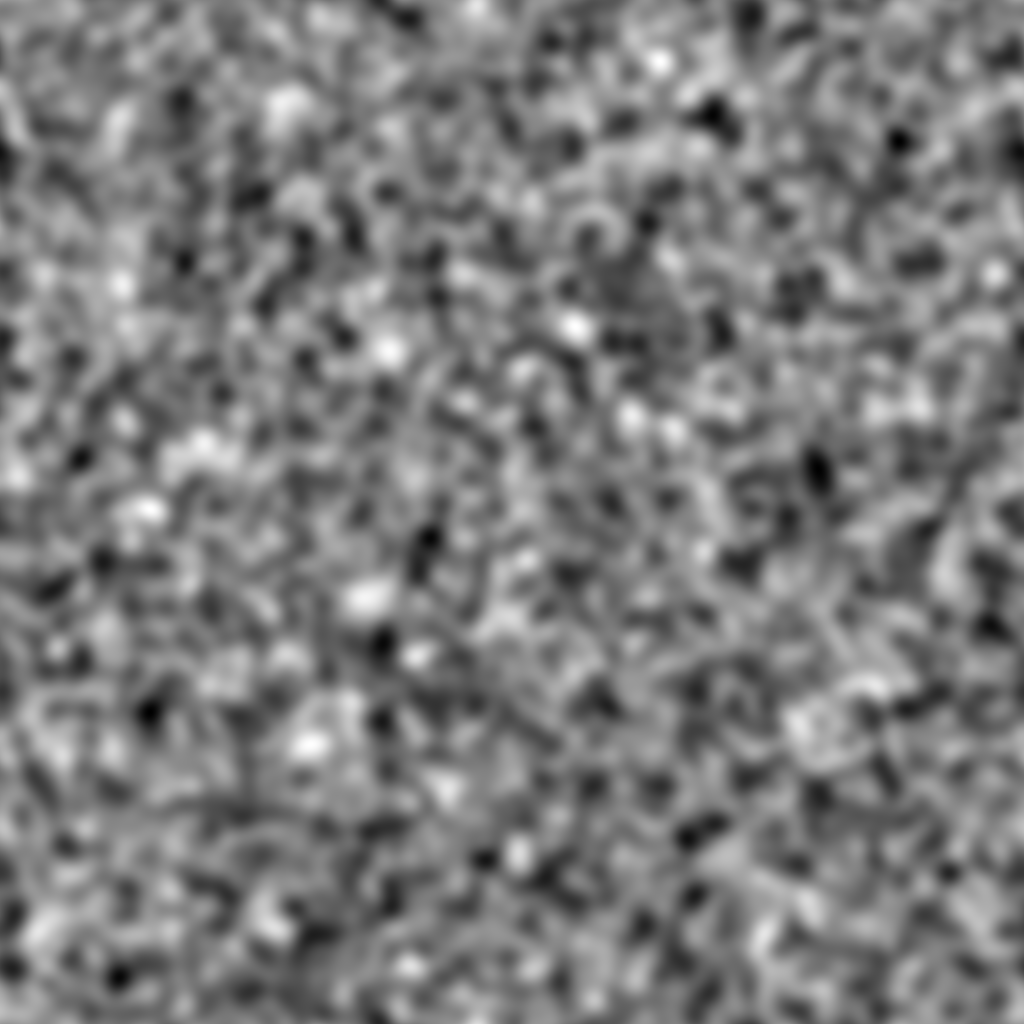
\includegraphics[width=5cm]{grf.python.png}%
 \label{fig:grf:python:grf}%
\end{figure}


\subsection{Minkowski functionals}

The Minkowski functionals are illustrated in Fig.\ref{fig:grf:python:Minkowski}. The code follows.

\begin{figure}[htbp]
 \centering\caption{Illustration of the simulated and analytical values of the Minkowski functionals of the level sets of the Gaussian Random Field, for $\sigma=10$ and $N=1024$.}%
 \subfloat[Area.]{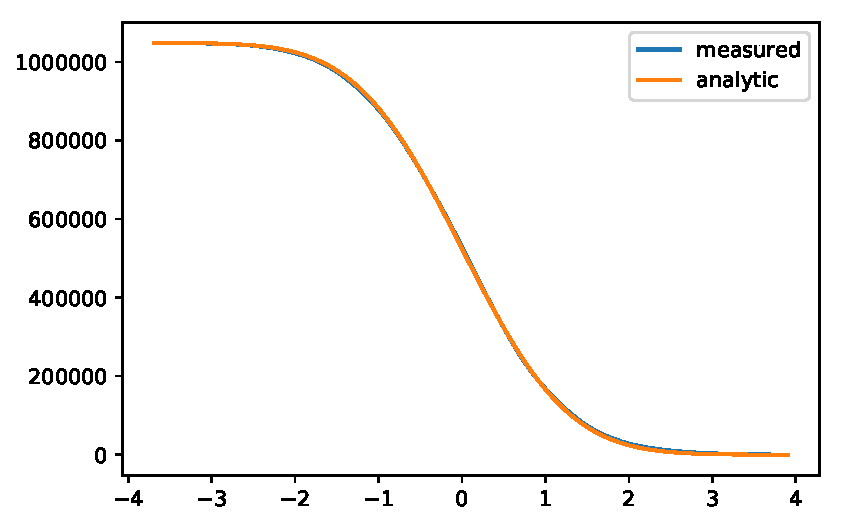
\includegraphics[width=.7\linewidth]{area.python.pdf}}
 
 \subfloat[Perimeter.]{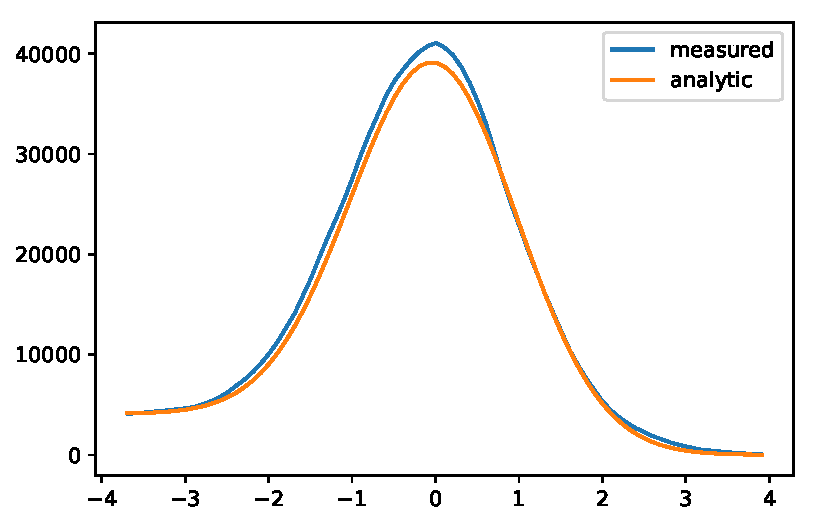
\includegraphics[width=.7\linewidth]{perimeter.python.pdf}}
 
 \subfloat[Euler number in 4 connecti\-vi\-ty.]{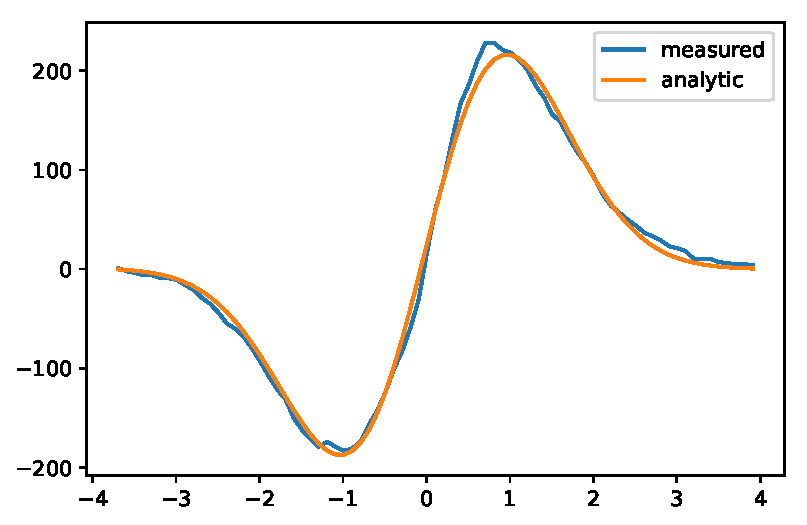
\includegraphics[width=.7\linewidth]{euler.python.pdf}}%
 \label{fig:grf:python:Minkowski}%
\end{figure}

The measures can be performed with the code from the tutorial \iflabelexists{tutorial:integral_geometry:enonce}{\ref{tutorial:integral_geometry:enonce}}{about integral geometry}.

\begin{python}
def bwminko(X):
    # zero padding of input
    X = np.pad(X, ((1,1), (1,1)), mode='constant');
    # Neighborhood configuration
    F = np.array([[0, 0, 0], [0, 1, 4], [0, 2, 8]]);
    XF = signal.convolve2d(X,F,mode='same');
    edges = np.arange(0, 17 ,1);
    h,edges = np.histogram(XF[:],bins=edges);
    
    f_intra = [0,1,0,1,0,1,0,1,0,1,0,1,0,1,0,1];
    e_intra = [0,2,1,2,1,2,2,2,0,2,1,2,1,2,2,2];
    v_intra = [0,1,1,1,1,1,1,1,1,1,1,1,1,1,1,1];
    f_inter = [0,0,0,0,0,0,0,0,0,0,0,0,0,0,0,1];
    e_inter = [0,0,0,1,0,1,0,2,0,0,0,1,0,1,0,2];
    v_inter = [0,1,0,1,0,1,0,1,0,1,0,1,0,1,0,1];
    EulerNb4 = np.sum(h*v_inter - h*e_inter + h*f_inter)
    Area = np.sum(h*f_intra)
    Perimeter = np.sum(-4*h*f_intra + 2*h*e_intra)
    return Area, Perimeter, EulerNb4;
\end{python}

Then, the measurements consists in taking all the level-sets and evaluating the properties from these binary sets. Notice that the perimeter is allways a difficult task and is not really precise.

\begin{python}
def minkoMeasured(G, sigma, hmin, hmax):
    H = np.arange(hmin, hmax, .1);
    A = [];
    P = [];
    E = [];
    bar = progressbar.ProgressBar();
    for h in bar(H):
        levelset = G >= h;
        a, p, e = bwminko(levelset); 
        A.append(a);
        P.append(p);
        E.append(e);
    return A, P, E;
\end{python}

The analytical values are simply evaluated with the formulas.
\begin{python}
def minkoAnalytical(N, sigma, hmin, hmax):
    l = 1/(2*sigma**2);
    # analytical values
    H = np.arange(hmin, hmax, .1);
    rho_0 = 1/2 * erfc(H / np.sqrt(2));
    rho_1 = np.sqrt(l) * np.exp(- H**2 / 2) /(2*np.pi);
    rho_2 = l / (2*np.pi)**(3/2) * np.exp(- H**2 / 2) * H;
    
    Aa = N**2 * rho_0;
    Pa = 4*N*rho_0 + np.pi*N**2*rho_1;
    Ea = rho_0 + 2*N*rho_1 + N**2*rho_2;
    return Aa, Pa, Ea;
\end{python}
